%%% Fiktivní kapitola s ukázkami tabulek, obrázků a kódu

\chapter{Tabulky, obrázky, programy, vzorce}

Používání tabulek a grafů/obrázků v~odborném textu má některá společná pravidla a~některá specifická. Tabulky a grafy/obrázky neuvádíme přímo do textu, ale umístíme je buď na samostatné stránky nebo na vyhrazené místo v~horní nebo dolní části běžných stránek. \LaTeX\ se o~umístění plovoucích grafů a tabulek postará automaticky.

Grafy/obrázky a tabulky se číslují a jsou vybaveny legendou. Legenda má popisovat obsah grafu či tabulky tak podrobně, aby jim čtenář rozuměl bez důkladného studování textu práce.

Na tabulku a graf/obrázek musí být v~textu číselný odkaz (lze důrazně doporučit dynamický mechanismus křížových referencí, jený je součástí \LaTeX u). Na příslušném místě textu pak shrneme ty nejdůležitější závěry, které lze z~tabulky či grafu učinit. Text by měl být čitelný a srozumitelný i~bez prohlížení tabulek a grafů a tabulky a grafy by měly být srozumitelné i~bez podrobné četby textu.

Na tabulky a grafy odkazujeme pokud možno nepřímo v~průběhu běžného
toku textu; místo \emph{\uv{Tabulka~\ref{tab03:Nejaka} ukazuje, že
    muži jsou v~průměru o~$9,9\,\rm kg$ těžší než ženy}} raději napíšeme
\emph{\uv{Muži jsou o~$9,9\,\rm kg$ těžší než ženy (viz
    tab.~\ref{tab03:Nejaka})}}.

\section{Tabulky}

\begin{table}[htbp!]

\centering
%%% Tabulka používá následující balíčky:
%%%   - booktabs (\toprule, \midrule, \bottomrule)
%%%   - dcolumn (typ sloupce D: vycentrovaná čísla zarovnaná na
%%%     desetinnou čárku
%%%     Všimněte si, že ve zdrojovém kódu jsou desetinné tečky, ale
%%%     tisknou se čárky.

\caption{Maximálně věrohodné odhady v~modelu M.}\label{tab03:Nejaka}
\begin{tabular}{lD{.}{,}{3.2}D{.}{,}{1.2}D{.}{,}{2.3}}
\toprule
               &                & \multicolumn{1}{c}{\textbf{Směrod.}}   &  \\
\textbf{Efekt} & \multicolumn{1}{c}{\textbf{Odhad}} & \multicolumn{1}{c}{\textbf{chyba}$^a$} & \multicolumn{1}{c}{\textbf{P-hodnota}} \\
\midrule
Abs. člen     & -10.01 & 1.01 & \multicolumn{1}{c}{---} \\
Pohlaví (muž) & 9.89   & 5.98 & 0.098 \\
Výška (cm)    & 0.78   & 0.12 & <0.001 \\
\bottomrule
\multicolumn{4}{l}{\footnotesize \textit{Pozn:}$^a$ Směrodatná chyba odhadu metodou Monte Carlo.}
\end{tabular}
\end{table}

U~\textbf{tabulek} se doporučuje dodržovat následující pravidla:

\begin{itemize} %% nebo compactitem z balíku paralist
\item Vyhýbat se svislým linkám. Silnějšími vodorovnými linkami
  oddělit tabulku od okolního textu včetně legendy, slabšími
  vodorovnými linkami oddělovat záhlaví sloupců od těla tabulky a
  jednotlivé části tabulky mezi sebou. V~\LaTeX u tuto podobu tabulek
  implementuje balík \texttt{booktabs}. Chceme-li výrazněji oddělit
  některé sloupce od jiných, vložíme mezi ně větší mezeru.
\item Neměnit typ, formát a význam obsahu políček v~tomtéž sloupci
  (není dobré do téhož sloupce zapisovat tu průměr, onde procenta).
\item Neopakovat tentýž obsah políček mnohokrát za sebou. Máme-li
  sloupec \textit{Rozptyl}, který v~prvních deseti řádcích obsahuje
  hodnotu $0,5$ a v~druhých deseti řádcích hodnotu $1,5$, pak tento
  sloupec raději zrušíme a vyřešíme to jinak. Například můžeme tabulku
  rozdělit na dvě nebo do ní vložit popisné řádky, které informují
o~nějaké proměnné hodnotě opakující se v~následujícím oddíle tabulky
  (např. \emph{\uv{Rozptyl${}=0,5$}} a níže \emph{\uv{Rozptyl${}=
      1,5$}}).
\item Čísla v~tabulce zarovnávat na desetinnou čárku.
\item V~tabulce je někdy potřebné používat zkratky, které se jinde
nevyskytují. Tyto zkratky můžeme vysvětlit v~legendě nebo
v~poznámkách pod tabulkou. Poznámky pod tabulkou můžeme využít i
k~podrobnějšímu vysvětlení významu  některých sloupců nebo hodnot.
\end{itemize}


\section{Obrázky}

\begin{figure}[htbp!]\centering
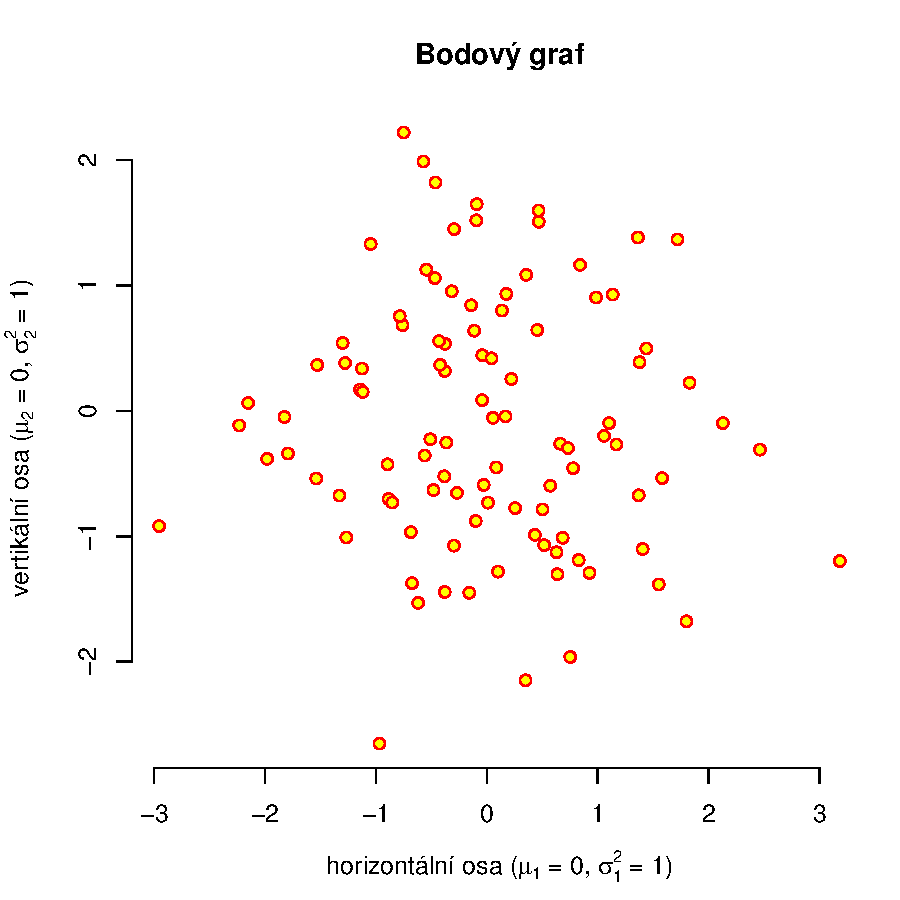
\includegraphics[width=.66\textwidth]{img/ukazka-obr01}
% Příponu není potřeba explicitně uvádět, pdflatex automaticky hledá pdf.
% Rozměry také není nutné uvádět.
\caption{Náhodný výběr z~rozdělení $\mathcal{N}_2(\boldsymbol{0},\,I)$.}
\label{obr03:Nvyber}
\end{figure}

Několik rad týkajících se obrázků a grafů.

\begin{itemize}
\item Graf by měl být vytvořen ve velikosti, v~níž bude použit
  v~práci. Zmenšení příliš velkého grafu vede ke špatné čitelnosti
  popisků.
\item Osy grafu musí být řádně popsány ve stejném jazyce, v~jakém je
  psána práce (absenci diakritiky lze tolerovat). Kreslíme-li graf
  hmotnosti proti výšce, nenecháme na nich popisky \texttt{ht} a
  \texttt{wt}, ale osy popíšeme \emph{Výška [cm]} a~\emph{Hmotnost
    [kg]}. Kreslíme-li graf funkce $h(x)$, popíšeme osy $x$ a $h(x)$.
  Každá osa musí mít jasně určenou škálu.
\item Chceme-li na dvourozměrném grafu vyznačit velké množství bodů,
  dáme pozor, aby se neslily do jednolité černé tmy. Je-li bodů mnoho,
  zmenšíme velikost symbolu, kterým je vykreslujeme, anebo vybereme
  jen malou část bodů, kterou do grafu zaneseme. Grafy, které obsahují
  tisíce bodů, dělají problémy hlavně v~elektronických dokumentech,
  protože výrazně zvětšují velikost souborů.
\item Budeme-li práci tisknout černobíle, vyhneme se používání barev.
  Čáry roz\-li\-šu\-je\-me typem (plná, tečkovaná, čerchovaná,\ldots), plochy
  dostatečně roz\-díl\-ný\-mi intensitami šedé nebo šrafováním. Význam
  jednotlivých typů čar a~ploch vysvětlíme buď v~textové legendě ke
  grafu anebo v~grafické legendě, která je přímo součástí obrázku.
\item Vyhýbejte se bitmapovým obrázkům o~nízkém rozlišení a zejména
  JPEGům (zuby a kompresní artefakty nevypadají na papíře pěkně).
  Lepší je vytvářet obrázky vektorově a vložit do textu jako PDF.
\end{itemize}


\section{Zdrojové kódy}
Algoritmy, výpisy programů a popis interakce s~programy je vhodné odlišit od ostatního textu. Jednou z~možností je použití {\LaTeX}o\-vé\-ho balíčku \texttt{listings}, pomocí něhož je v~souboru \texttt{makra.tex} nadefinováno jednoduché prostředí \texttt{code}. Pomocí něho lze vytvořit např. následující ukázky.

\begin{code}
> mean(x)
[1] 158.90
> objekt$prumer
[1] 158.90
\end{code}

Balíček \texttt{listings} a jeho prostředí \texttt{lstlisting} však nabízí téměř nepřeberné množství konfiguračních parametrů, např. pro zvýrazňování syntaxe programovacích jazyků (několika desítek), číslování řádku atd. Příklady:
\begin{itemize}
\item \url{https://en.wikibooks.org/wiki/LaTeX/Source_Code_Listings}
\item \url{https://www.overleaf.com/learn/latex/Code_listing#Using_listings_to_highlight_code}
\end{itemize}


\section{Sazba matematiky}
Proměnné sázíme kurzívou (to \TeX{} v~matematickém módu dělá sám, ale
nezapomínejte na to v~okolním textu a také si matematický mód zapněte).
Názvy funkcí sázíme vzpřímeně. Tedy například:
$\textrm{var} (X) = \textsf{E~} X^2 - \bigl(\textsf{E~} X \bigr)^2$.

Zlomky uvnitř odstavce (třeba $\frac{5}{7}$ nebo $\frac{x+y}{2}$) mohou
být příliš stísněné, takže je lepší sázet jednoduché zlomky s~lomítkem:
$5/7$, $(x+y)/2$.

Pro méně obeznámené se zvyklostmi v matematické sazbě lze doporučit stručný text od Richarda Starého -- \url{http://richardstary.wz.cz/clanky/matsaz/matsaz.pdf} --, který je obecně platný bez ohledu na to, zda použijete \LaTeX\ nebo Word.

Možnosti \LaTeX u pro sazbu matematiky jsou sice bohaté, ale je možné, že v některých specifických situacích nebudou postačovat. Proto lze doporučit k použití balíčky American Mathematical Society (AMS). V souboru \texttt{makra.tex} jsou standardně zaváděny balíčky \texttt{amsmath}, \texttt{amsfonts} a \texttt{amsthm}. Pro proniknutí do jejich možností poslouží:
\begin{itemize}
\item Math Extension with AMS\LaTeX\ -- \url{http://ptgmedia.pearsoncmg.com/images/0321173856/samplechapter/kopkach15.pdf}
\item \url{https://www.overleaf.com/learn/latex/Aligning_equations_with_amsmath}
\item Math Mode -- \url{http://tex.loria.fr/general/Voss-Mathmode.pdf}
\item More Math into LaTeX -- \url{http://tug.ctan.org/info/Math_into_LaTeX-4/Short_Course.pdf}
\end{itemize}

Ukázka číslovaného vzorce:
\begin{equation}
\mathbf{b}=(\mathbf{X}^\mathsf{T}\mathbf{X})^{-1}\mathbf{X}^\mathsf{T}\mathbf{y}
\end{equation}

Ukázka nečíslovaných vzorců s funkcemi a indexy:

$$
d_{ij}=\max_{k=1,2,\dots,n} \{d_{ik}+d_{kj}\},
$$
$$
x_{1,2}=b \pm \sqrt{\ln y}.
$$

Ukázku vzorce jako součást jednoho odstavce uveďme na příkladu kapacit dodavatelů v matematickém modelu dopravního problému, které zohledníme pomocí omezení:
\begin{equation}
\sum_{j=1}^n x_{ij} \le a_i, \qquad i=1,2,\dots,m\ ,
\end{equation}
\noindent
kde výraz $a_i$ představuje kapacitu $i$-tého dodavatele.

Při odvozování vzorce postupnou úpravou se obvykle jednotlivé kroky uvádějí na samostatných řádcích (prostředí \verb'align*' z balíčku \verb|amsmath|):
\begin{align*}
 f(x) &= (x+a)(x+b) =\\
      &= x^2 + bx + ax + ab =\\
      &= x^2 + (a+b)x + ab
\end{align*}

Ukázka sloupcové úpravy (\verb|eqnarray*|):
\begin{eqnarray*}
\sum_{i=1}^n x_{ij} =1, && j=1,2,\dots,n,\\
\sum_{j=1}^n x_{ij} =1, && i=1,2,\dots,n,\\
u_i + 1 - M(1 - x_{ij}) \le u_j, && i=2,3,\dots,n,\quad j=1,2,\dots,n,\\
u_i \ge 0,              && i=1,2,\dots,n,\\
x_{ij} \in \{0,1\} && i=1,2,\dots,n,\quad j=1,2,\dots,n,\\
\end{eqnarray*}